\documentclass[a4paper,12pt]{report}
%general packages
\usepackage[T2A]{fontenc}
\usepackage[utf8]{inputenc}
\usepackage[english,russian]{babel}
\usepackage{circuitikz}
\usepackage{wrapfig}
\usepackage{makecell}
\usepackage{tabularx}
\usepackage{graphicx}
\usepackage{gensymb}
\usepackage{cancel} %cancel symbol
\usepackage{amsmath,amsfonts,amssymb,amsthm,mathtools}

%fancy header + geometry
\usepackage{fancyhdr}
\usepackage[a4paper,includehead,nomarginpar,left=15mm,right=15mm,top=15mm,headheight=10mm,bottom=20mm]{geometry}

%pgfplots
\usepackage{pgfplots}
\usepackage{pgfkeys}
\pgfplotsset{compat=1.12}
\usepackage{mathrsfs}

%multi column text
\usepackage{blindtext}
\usepackage{multicol}

%tikz (draw)
\usepackage{tikz}
\usepackage{pstricks-add}
\usetikzlibrary{intersections}
\usetikzlibrary{arrows.meta}
\usetikzlibrary{calc,angles,positioning}
\usetikzlibrary{arrows}
\usepackage{float}

%parskip settings
\parindent=0ex
\setlength{\parskip}{\baselineskip}%
\setlength{\parindent}{0pt}%

%fancy notation for sets
\newcommand{\R}{{\mathbb R}}
\newcommand{\N}{{\mathbb N}}
\newcommand{\fancy}[1]{{\mathbb{#1}}}
%sgn function
\DeclareMathOperator{\sgn}{sgn}

% intersection and union symbols
\newcommand{\uni}{\cup}
\newcommand{\inter}{\cap}

\renewcommand{\footrulewidth}{0.4pt}

%\newcommand{\celsius}{$\ ^\circ C$}

%environments

\newtheorem{problem}{Задача}[]
\newenvironment{sol}{\paragraph{Решение}}{}
\renewcommand\thesection{\arabic{section}}

\usepackage{titlesec}
\titlespacing*{\section}
{0pt}{\baselineskip}{0pt}
\titlespacing*{\paragraph}
{0pt}{\baselineskip}{\baselineskip}
\titlespacing*{\paragraph}
{0pt}{0.1\baselineskip}{\baselineskip}

\begin{document}
	

\begin{titlepage}
	\begin{center}
		МОСКОВСКИЙ ФИЗИКО-ТЕХНИЧЕСКИЙ ИНСТИТУТ (НАЦИОНАЛЬНЫЙ ИССЛЕДОВАТЕЛЬСКИЙ УНИВЕРСИТЕТ) \\
		
		
		\hfill \break
		Факультет обшей и прикладной физики\\
		\vspace{2.5cm}
		\large{\textbf{Отчёт по лабораторной работе 1.2.5 <<Исследование прецессии уравновешенного гороскопа>>}}\\
		\hfill \break
		\\
	\end{center}
	
	\begin{flushright}
		Выполнил:\\
		Студент гр. Б02-304\\
		Головинов. Г.А.
	\end{flushright}
	
	\vspace{7cm}
	
	\begin{center}
		
\includegraphics[width=0.15\linewidth]{uni}
	\end{center}
	

	

	\vfill
	
	\begin{center} Долгопрудный, 2023 \end{center}
	
	\thispagestyle{empty}
	
\end{titlepage}


	\newpage
	%\pagenumbering{arabic}
    \pagestyle{fancy}

    \fancyhead{}
    \fancyfoot{}
    \fancyhead[L]{\rightmark}
    \fancyhead[R]{\thepage}
    \fancyfoot[R]{Работа 2.1.6 --- Эффект Джоуля---Томсона}

    \section*{Аннотация}
        \paragraph*{Цель работы:} 1) определить изменения температуры углекислого газа при протекании через малопроницаемую перегородку при разных начальных значениях давления и температуры; 2) вычислить по результатам опытов коэффициенты $a$ и $b$ модели Ван-дер-Ваальса.
        \paragraph*{В работе используются:} трубка с пористой перегородкой; труба Дьюара; термостат жидкостный; дифференциальная термопара; мультиметр; балластный баллон; манометр.
    \vspace{0.5cm}
    \begin{multicols}{2}
    \section{Основные теоретические сведения}
        Эффектом Джоуля---Томсона называется изменение температуры газа, просачивающегося из области высокого в область низкого давления в условиях тепловой изоляции. В разреженных газах (практически идеальных) при таком течении температура не меняется.

        В работе газ из области повышенного давления $p_1$ проходит через множество узких и длинных каналов пористой перегородки в область с атмосферным давлением $p_2$. Перепад давления $|\Delta p|=p_1-p_2$ из-за большого сопротивления перегородки может быть заметным даже при малой скорости течения газа. Величина эффекта определяется по разности температур газа $\Delta T$ до и после перегородки.

        \paragraph*{Вывод эффекта Джоуля---Томсона.} Пусть через трубку прошел $\Delta \nu = 1$ mol. газа, пусть $V_1$ и $V_2$ --- молярные объемы газа до и после, $p_1$, $p_2$ --- соответствующие давления. $U_1$, $U_2$ --- внутренние энергии в расчете на 1 mol. Для того чтобы ввести в трубку порцию газа объемом $V_1$ необходимо совершить работу $A_1=p_1V_1$. Выходя из трубки эта же порция совершает работу $A_2=p_2V_2$. Считая, что стенки не проводят тепло и не совершается механической передачи энергии, получаем:
        \begin{align}
            A_1-A_2=p_1V_1-p_2V_2=\nonumber\\
            =(U_2+\mu v_2^2/2)-(U_1+\mu v_1^2/2)
            \label{dA}
        \end{align}
        здесь кроме изменения внутренней энергии $\Delta U$ учтена кинетическая энергия течения $\mu v_{1,2}^2/2$.

        Определим \emph{молярную энтальпию} газа как $H=U+pV$. Тогда уравнение \eqref{dA} можно переписать:
        \begin{equation}
            H_1-H_2=\frac{\mu}{2}(v_2^2-v_1^2)
            \label{dH}
        \end{equation}
        Это есть уравнение бернулли для течения газа, учитывающее его сжимаемость и внутреннюю энергию.
        
        Внутри перегородки газ испытывает трение. Это приводит к необратимому переходу почти всей кинетической энергии газа в тепловую. Теплообмена с окружающей средой нет, поэтому вся энергия отдается обратно газу и уносится с потоком. Закон сохранения энергии \eqref{dH} остается в силе, однако кинетическая энергия оказывается пренебрежимо малой. Приходим к выводу, что эффект Джоуля---Томсона --- это процесс, в котором энтальпия сохраняется:
        \begin{equation}
            \label{H1=H2}
            H_1\approx H_2
        \end{equation}
        Энтальпия --- функция состояния, зависящая от температуры и от давления. Коэффициентом Джоуля---Томсона называют отношение:
        \begin{equation}
            \label{coefD-T}
            \mu_{\text{J---T}}=\frac{\Delta T}{\Delta p}
        \end{equation}

        Эффект Джоуля---Томсона используется для получения низких температур, поэтому понижение температуры считается <<положительным эффектом>>.

        \paragraph*{Газ Ван-Дер-Ваальса.} В реальном газе внутренняя энергия зависит не только от температуры, но и от плотности газа: $U(T,V)$. Поэтому внешняя работа частично идет также на изменение внутренней энергии газа, что сопровождается изменением температуры. Рассмотрим модель реального газа: газ Ван-дер-Ваальса. Для него уравнения состояния:
        \begin{gather*}
            \left(p+\frac{a}{V^2}\right)(V-b)=RT,\\ 
            U=C_V T - \frac{a}{V}.
        \end{gather*}  
        Теплоемкость газа $C_V$ будем для простоты считать неизменной. Константа $a$ отвечает за притяжение полекул на дальних расстояниях, а константа $b$ отвечает за отталкивание на малых расстояниях. Имеет смысл минимально возможного молярного объема газа. Энтальпия Ван-Дер-Ваальса:
        \begin{equation}
            H=U+pV=C_V T + RT \frac{V}{V-b}-\frac{2a}{V}
        \end{equation}
        Формула не совсем удобна, поэтому для упрощения стоит воспользоваться тем, что газ в опыте достаточно разрежен. Давление не превышает 5 bar. Его поведение достаточно близко к идеальному, поэтому отличия от идеального стоит учитывать только в эффекте Джоуля---Томсона. С учетом, что $C_V+R\approx C_p$ получится:
        \begin{equation}
            H \approx C_p T + p \left(b-\frac{2a}{RT}\right)
        \end{equation}
        Также примем, что изменение температуры в опыте мало: $\Delta T/T \ll 1$. Тогда полагая $\Delta H = 0$ для предыдущего уравнения получим окончательное выражение для коэффициента Джоуля---Томсона:
        \begin{equation}
            \label{j-tfinal}
            \mu_{\text{J---T}}=-\frac{\Delta T}{\Delta p}\approx -\frac{b-2a/RT}{C_p}
        \end{equation}
        \paragraph*{Температура инверсии.} Из окончательного соотношения для коэффициента $\mu_{\text{J---T}}$ видно, что есть некоторая температура, при которой знак изменения температуры меняется:
        \begin{equation*}
            T_\text{inv}=\frac{2a}{Rb}
        \end{equation*}
        При $T>T_\text{inv}$ газ нагревается, т.е. $\mu < 0$, а при $T>T_\text{inv}$ наоборот, охлаждается ($\mu > 0$). Для углекислого газа $\text{CO}_2$ температура инверсии $T_\text{inv}\sim 1500\ \text{K}$ при давлении $p \sim 1 \ \text{bar}$, то есть при комнатной температуре газ будет охлаждаться, $\mu > 0$.
    \end{multicols}
    \newpage
    \section{Экспериментальная установка.}
        Схема установки представлена на Рис.~\ref{fig:1}. Основным элементов является трубка 1 с пористой перегородкой 2, через которую пропускается газ. Трубка имеет длину 80 mm и сделана из нержавеющей стали, поэтому имеет малую теплопроводность. Диаметр трубки $d=3$ mm, толщина стенок $0.2$ mm. Пористая перегородка расположена в конце трубки и представляет собой стеклянную пористую пробку. Пористость и толщина перегородки подобрана так, чтобы обеспечить оптимальный поток газа при разнице давлений $\Delta p \leq 4$ bar.
        \begin{figure}[H]
            \centering
            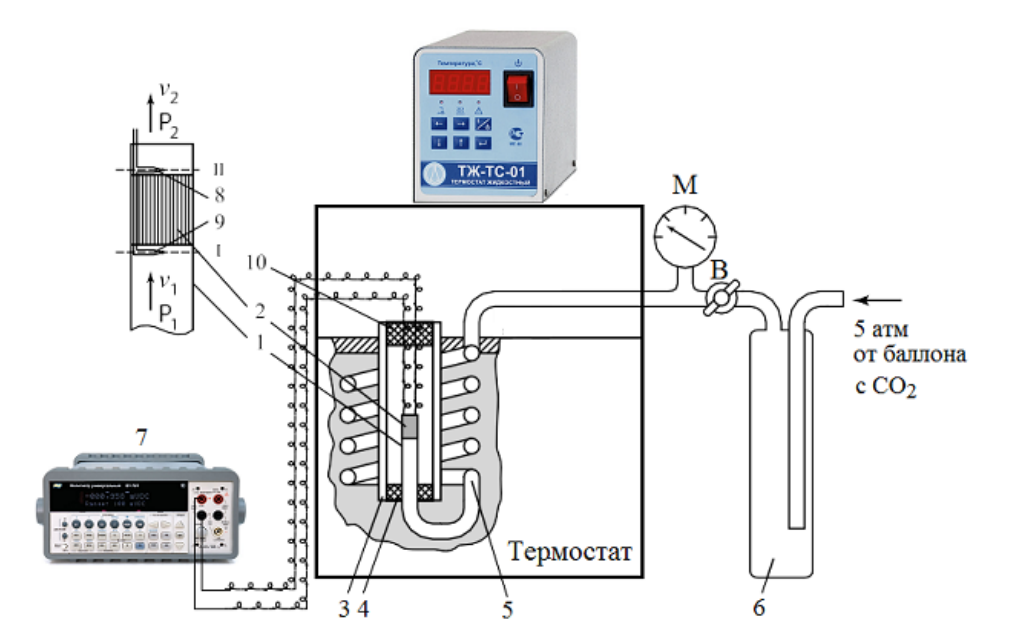
\includegraphics[width=0.9\linewidth]{../img/ustanovka.png}
            \caption{Схема экспериментальной установки}
            \label{fig:1}
        \end{figure}
        Углекислый газ подается под давлением через змеевик 5 из баллона 6. Бедный змеевик омывается водой и нагревает газ до температуры воды в термостате.

        Давление газа измеряется манометром М и регулируется вентилем В. Манометр показывает разницу между давлением внутри трубки и атмосферой. Поэтому нормальное показание манометра равно нулю.

        Разность температур газа до и после перегородки измеряется дифференциальной термопарой медь---константан. С помощью вольтметра 7 измеряется разность потенциалов $V$, которая возникает из-за разницы температур. Зависимость $V(t)$ не является линейной, однако в этой работе измеряются малые перепады температур, поэтому этим можно пренебречь. Чувствительность термопары также зависит от температуры, поэтому нам была предоставлена таблица коэффициентов $dV/dt$ для разных температур.
    
    \newpage
    \begin{multicols}{2}
    \section{Обработка результатов измерений}
        В результате измерений были получены данные для 4-х различных температур. Для каждой температуры были измерены разницы потенциалов $V$ (которые впоследствии будут переведены в разность температур $\Delta T$) при различных перепадах давления в промежутке от $p=1.5$ bar до $p=4$ bar. Таблицы с полученными данными приведены в приложении.
        
        Величина показания вольтметра в отсутствие потока газа  (постоянные паразитические эффекты) была пренебрежима мала, поэтому не учитывалась.

        Отложив полученные значения по наклону прямой $\Delta T (\Delta p)$ можно определить значения коэффициента $\mu_{\text{J---T}}$.
    \end{multicols}
    \begin{figure}[H]
        \centering
        \begin{tikzpicture}[scale=0.8]
            \begin{axis}[
                name=plot1,
                ymajorgrids=true,
                xmajorgrids=true,
                title={$\Delta T (\Delta p)$,\ $T=30\ \celsius$},
                xlabel={$\Delta p, \ \text{bar}$},
                ylabel={$\Delta T, \ \celsius$},
                legend pos = south west,
                legend style={nodes={scale=1, transform shape}}, 
                %legend image post style={mark=*},
            ]
            \addplot[
                only marks,mark=*,color=black,mark size = 1pt
            ]
            plot [error bars/.cd, y dir = both, x dir = both, y explicit, x explicit]
            table[meta=label, x=dP, y=dT, x error = eP, y error=eT]{
                dP	dT	eP	eT	label
                4	-3.844282238	0.1	0.0486618	1
                3.5	-3.309002433	0.1	0.0486618	2
                3	-2.749391727	0.1	0.0486618	3
                2.5	-2.238442822	0.1	0.0486618	4
                2	-1.703163017	0.1	0.0486618	5
                1.5	-1.216545012	0.1	0.0486618	6

            };
            \addlegendentry[]{Experimental}
            \addplot[color=blue,domain=1:4.5] {-0.925307804*x};
            \addlegendentry[]{Approximation}
            \end{axis}
            
            \begin{axis}[
                name=plot2,
                xshift=1cm,
                at=(plot1.outer south east),
                anchor=outer south west,
                title={$\Delta T (\Delta p)$,\ $T=40\ \celsius$},
                ymajorgrids=true,
                xmajorgrids=true,
                xlabel={$\Delta p, \ \text{bar}$},
                ylabel={$\Delta T, \ \celsius$},
                legend pos = south west,
                legend style={nodes={scale=1, transform shape}}, 
                %legend image post style={mark=*},
            ]
            \addplot[
                only marks,mark=*,color=black,mark size = 1pt
            ]
            plot [error bars/.cd, y dir = both, x dir = both, y explicit, x explicit]
            table[meta=label, x=dP, y=dT, x error = eP, y error=eT]{
                dP	dT	eP	eT	label
                4	-3.57568534	0.1	0.047675805	1
                3.5	-3.05125149	0.1	0.047675805	2
                3	-2.550655542	0.1	0.047675805	3
                2.5	-2.121573302	0.1	0.047675805	4
                2	-1.525625745	0.1	0.047675805	5
                1.5	-1.072705602	0.1	0.047675805	6
                

            };
            \addlegendentry[]{Experimental}
            \addplot[blue,domain=1:4.5] {-0.856247866*x};
            \addlegendentry{Approximation}
            \end{axis}

            \begin{axis}[
                name=plot3,
                yshift=-1cm,
                at=(plot1.outer south east),
                anchor=outer north east,
                title={$\Delta T (\Delta p)$,\ $T=50\ \celsius$},
                ymajorgrids=true,
                xmajorgrids=true,
                xlabel={$\Delta p, \ \text{bar}$},
                ylabel={$\Delta T, \ \celsius$},
                legend pos = south west,
                legend style={nodes={scale=1, transform shape}}, 
                %legend image post style={mark=*},
            ]
            \addplot[
                only marks,mark=*,color=black,mark size = 1pt
            ]
            plot [error bars/.cd, y dir = both, x dir = both, y explicit, x explicit]
            table[meta=label, x=dP, y=dT, x error = eP, y error=eT]{
                dP	dT	eP	eT	label
                4	-3.317757009	0.1	0.046728972	1
                3.5	-2.803738318	0.1	0.046728972	2
                3	-2.38317757	0.1	0.046728972	3
                2.5	-1.892523364	0.1	0.046728972	4
                2	-1.448598131	0.1	0.046728972	5
                1.5	-1.028037383	0.1	0.046728972	6


            };
            \addlegendentry[]{Experimental}
            \addplot[blue,domain=1:4.5] {-0.792044334*x};
            \addlegendentry{Approximation}
            \end{axis}

            \begin{axis}[
                name=plot3,
                yshift=-1cm,
                xshift=1cm,
                at=(plot1.outer south east),
                anchor=outer north west,
                title={$\Delta T (\Delta p)$,\ $T=60\ \celsius$},
                ymajorgrids=true,
                xmajorgrids=true,
                xlabel={$\Delta p, \ \text{bar}$},
                ylabel={$\Delta T, \ \celsius$},
                legend pos = south west,
                legend style={nodes={scale=1, transform shape}}, 
                %legend image post style={mark=*},
            ]
            \addplot[
                only marks,mark=*,color=black,mark size = 1pt
            ]
            plot [error bars/.cd, y dir = both, x dir = both, y explicit, x explicit]
            table[meta=label, x=dP, y=dT, x error = eP, y error=eT]{
                dP	dT	eP	eT	label
                4	-3.092783505	0.1	0.045819015	1
                3.5	-2.611683849	0.1	0.045819015	2
                3	-2.199312715	0.1	0.045819015	3
                2.5	-1.809851088	0.1	0.045819015	4
                2	-1.328751432	0.1	0.045819015	5
                1.5	-1.008018328	0.1	0.045819015	6
                
            };
            \addlegendentry[]{Experimental}
            \addplot[blue,domain=1:4.5] {-0.739781381*x};
            \addlegendentry{Approximation}
            \end{axis}
        \end{tikzpicture}
        \caption{Полученные точки и аппроксимация зависимости методом МНК.}
    \end{figure}
    Как видно, точки хорошо ложатся на прямую во всех четырех случаях. По методу МНК проведем прямые и возьмем коэффициенты наклона $k=\mu_{\text{J---T}}$ для каждой температуры. Изменение температуры в данном случае отрицательное, это зависит от полярности термопары, которая в данном случае подключена таким образом, что $\Delta T=T_\text{out}-T_\text{in}$, то есть показывает <<положительный>> эффект Джоуля---Томсона.
    \newpage

    \begin{multicols}{2}
        Методом МНК получены коэффициенты наклона $k$ для каждой температуры:
        \begin{align*}
            k_1=(-0.925\pm 0.018)\ \text{K}/\text{bar}\\
            k_2=(-0.856\pm 0.021)\ \text{K}/\text{bar}\\
            k_3=(-0.792\pm 0.017)\ \text{K}/\text{bar}\\
            k_4=(-0.740\pm 0.015)\ \text{K}/\text{bar}
        \end{align*}
        Полученные значения близки к табличным (порядка 0.7---0.8 при 40---60 $\celsius$ при 1 bar).

        Важно заметить, что аппроксимация не совсем ложится на прямую, так как при отсутствующей разнице давлений наблюдалось отсутствие разницы температур, поэтому аппроксимация осуществлялась прямой $y=kx$.

        Теперь построим зависимость $\mu_\text{J---T}(1/T)$. Она должна быть линейной. Из этой зависимости мы можем определить постоянные $a$ и $b$ в модели газа Ван-Дер-Ваальса.
        \begin{figure}[H]
            \centering
            \begin{tikzpicture}[scale=1]
                \begin{axis}[
                    name=plot1,
                    ymajorgrids=true,
                    xmajorgrids=true,
                    title={$\mu_\text{J---T}(1/T)$},
                    xlabel={$1/T, \ \text{K}^{-1}$},
                    ylabel={$\mu_\text{J---T},\ \text{K}/\text{bar}$},
                    legend pos = north west,
                    legend style={nodes={scale=1, transform shape}}, 
                    %legend image post style={mark=*},
                ]
                \addplot[
                    only marks,mark=*,color=black,mark size = 1pt
                ]
                plot [error bars/.cd, y dir = both, x dir = both, y explicit, x explicit]
                table[meta=label, x=1/T, y=mu, x error = sigmaT, y error=sigmamu]{
                    1/T	mu	sigmamu	sigmaT	label
                    0.00330033	0.925307804	0.01825032	1.10011E-05	1
                    0.003194888	0.856247866	0.02065064	7.98722E-06	2
                    0.003095975	0.792044334	0.01737089	6.19195E-06	3
                    0.003003003	0.739781381	0.014653871	5.00501E-06	4

                        
                };
                \addlegendentry[]{Experimental}
                \addplot[color=blue,domain=2.97E-3:3.33E-3] {627.053*x-1.14596};
                \addlegendentry[]{Approximation}
                \end{axis}
            \end{tikzpicture}
            \caption{Зависимость коэффициента Джоуля---Томсона от температуры.}
        \end{figure}
        Точки хорошо ложатся на прямую. Будем аппроксимировать по МНК прямой $y=Kx+B$.

        Коэффициент наклона, согласно теории, равен:
        \begin{equation*}
            K=\frac{1}{C_p}\cdot \frac{2a}{R}
        \end{equation*}
        Координата по $y$ точки пересечения с осью ординат $B$ равна:
        \begin{equation*}
            B=-\frac{b}{C_p}
        \end{equation*}
        Получили $K=627.05$, $B=-1.14$. В нашем диапазоне температур $C_p$ углекислого газа $\approx 860\ \text{J}/\text{kg}\ \celsius$. Полученные значения соответствуют следующим значениям постоянных модели Ван-Дер-Ваальса:
        \begin{gather*}
            b\approx 431.38 \  \frac{\text{cm}^3}{\text{mol}}\\
            a\approx 0.99 \ \frac{\text{N}\cdot \text{m}^4}{\text{mol}^2}
        \end{gather*}

        Пересечение графика с осью абсцисс наблюдается при $1/T=0.0183$, что дает температуру порядка $550$ K. Это намного ниже теоретической оценки более тысячи К.

        Полученные значения значительно отличаются от табличных.
        \section{Обсуждение результатов и выводы.}
        В результате работы получены зависимости изменения температуры вследствие эффекта Джоуля---Томсона от разницы давления при различных температурах. Полученные зависимости оказались линейными, коэффициент их наклона есть искомый коэффициент Джоуля---Томсона. Полученные значения хорошо соотносятся с табличными.

        При экстраполяции полученных коэффициентов Джоуля---Томсона от температуры получены постоянные $a$, $b$ модели газа Ван-Дер-Ваальса, а также получена оценка температуры инверсии $T_\text{inv}$. Полученные значения достаточно сильно отличаются от табличных, что говорит о несовершенстве модели.
    \end{multicols}
    \newpage
    \section{Приложение}
    \begin{figure}[H]
        \centering
        \begin{tabular}{|c|c|c|c|c|c|c|}
            \hline
            $\Delta p$, bar & 4 & 3.5 & 3 & 2.5 & 2 & 1.5 \\
            \hline
            $\Delta V, \ \mu$V & -150 & -128 & -107 & -89 & -64 & -45 \\
            \hline
            $\Delta V/\Delta T$, $\mu\text{V}$/K & 41.95 & 41.95 & 41.95 & 41.95 & 41.95 & 41.95 \\
            \hline
            $\Delta T,$ K & -3.58 & -3.05 & -2.55 & -2.12 & -1.53 & -1.07 \\
            \hline
        \end{tabular}
        \caption{Результаты измерений при $T=30$ \celsius}
    \end{figure}
    \begin{figure}[H]
        \centering
        \begin{tabular}{|c|c|c|c|c|c|c|}
            \hline
            $\Delta p$, bar & 4 & 3.5 & 3 & 2.5 & 2 & 1.5 \\
            \hline
            $\Delta V, \ \mu$V & -142 & -120 & -102 & -81 & -62 & -44 \\
            \hline
            $\Delta V/\Delta T$, $\mu\text{V}$/K & 42.8 & 42.8 & 42.8 & 42.8 & 42.8 & 42.8 \\
            \hline
            $\Delta T,$ K & -3.32 & -2.80 & -2.38 & -1.89 & -1.45 & -1.03 \\
            \hline
        \end{tabular}
        \caption{Результаты измерений при $T=40$ \celsius}
    \end{figure}
    \begin{figure}[H]
        \centering
        \begin{tabular}{|c|c|c|c|c|c|c|}
            \hline
            $\Delta p$, bar & 4 & 3.5 & 3 & 2.5 & 2 & 1.5 \\
            \hline
            $\Delta V, \ \mu$V & -135 & -114 & -96 & -79 & -58 & -44 \\
            \hline
            $\Delta V/\Delta T$, $\mu\text{V}$/K & 43.65 & 43.65 & 43.65 & 43.65 & 43.65 & 43.65 \\
            \hline
            $\Delta T,$ K & -3.09 & -2.61 & -2.20 & -1.81 & -1.33 & -1.01 \\
            \hline
        \end{tabular}
        \caption{Результаты измерений при $T=50$ \celsius}
    \end{figure}
    \begin{figure}[H]
        \centering
        \begin{tabular}{|c|c|c|c|c|c|c|}
            \hline
            $\Delta p$, bar & 4 & 3.5 & 3 & 2.5 & 2 & 1.5 \\
            \hline
            $\Delta V, \ \mu$V & -158 & -136 & -113 & -92 & -70 & -50 \\
            \hline
            $\Delta V/\Delta T$, $\mu\text{V}$/K & 41.1 & 41.1 & 41.1 & 41.1 & 41.1 & 41.1 \\
            \hline
            $\Delta T,$ K & -3.84 & -3.31 & -2.75 & -2.24 & -1.70 & -1.22 \\
            \hline
        \end{tabular}
        \caption{Результаты измерений при $T=60$ \celsius}
    \end{figure}
\end{document}
